\begin{center}
    

\tikzset{every picture/.style={line width=0.75pt}} %set default line width to 0.75pt        

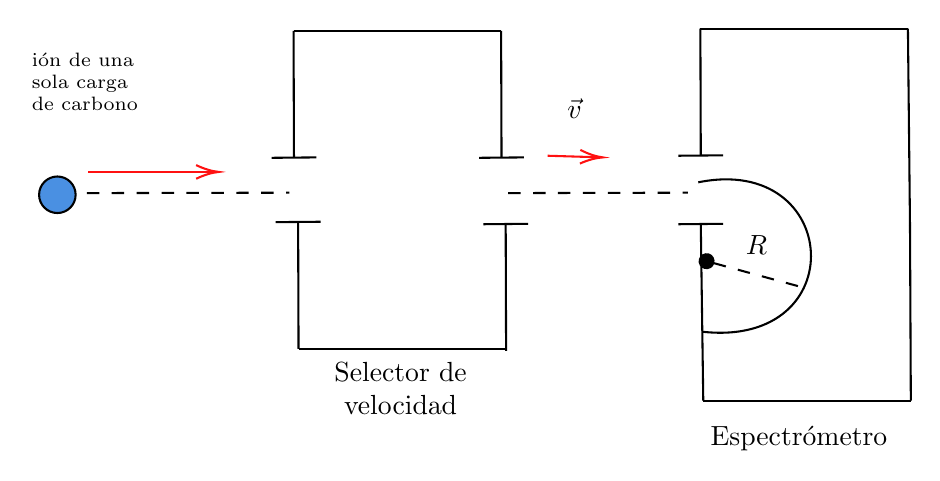
\begin{tikzpicture}[x=0.75pt,y=0.75pt,yscale=-1,xscale=1]
%uncomment if require: \path (0,350); %set diagram left start at 0, and has height of 350

%Shape: Circle [id:dp6869499625868678] 
\draw  [fill={rgb, 255:red, 74; green, 144; blue, 226 }  ,fill opacity=1 ] (66,157.8) .. controls (66,152.94) and (69.94,149) .. (74.8,149) .. controls (79.66,149) and (83.6,152.94) .. (83.6,157.8) .. controls (83.6,162.66) and (79.66,166.6) .. (74.8,166.6) .. controls (69.94,166.6) and (66,162.66) .. (66,157.8) -- cycle ;
%Straight Lines [id:da9745963202631923] 
\draw [color={rgb, 255:red, 255; green, 17; blue, 17 }  ,draw opacity=1 ]   (89.6,146.8) -- (150.6,146.8) ;
\draw [shift={(152.6,146.8)}, rotate = 180] [color={rgb, 255:red, 255; green, 17; blue, 17 }  ,draw opacity=1 ][line width=0.75]    (10.93,-3.29) .. controls (6.95,-1.4) and (3.31,-0.3) .. (0,0) .. controls (3.31,0.3) and (6.95,1.4) .. (10.93,3.29)   ;
%Straight Lines [id:da12352787521842434] 
\draw  [dash pattern={on 4.5pt off 4.5pt}]  (89,157) -- (186.6,156.8) ;
%Straight Lines [id:da5324098897262721] 
\draw    (178,140) -- (199.6,139.8) ;
%Straight Lines [id:da756451472892946] 
\draw    (180,171) -- (201.6,170.8) ;
%Straight Lines [id:da15776838209472221] 
\draw    (278,140) -- (299.6,139.8) ;
%Straight Lines [id:da72273411804861] 
\draw    (280,172) -- (301.6,171.8) ;
%Straight Lines [id:da8068958588484031] 
\draw    (188.6,78.8) -- (188.8,139.9) ;
%Straight Lines [id:da09923472401685407] 
\draw    (288.6,78.8) -- (288.8,139.9) ;
%Straight Lines [id:da9166512618354345] 
\draw    (190.8,170.9) -- (191,232) ;
%Straight Lines [id:da2811225134163712] 
\draw    (290.8,171.9) -- (291,233) ;
%Straight Lines [id:da37337061431721763] 
\draw    (188.6,78.8) -- (288.6,78.8) ;
%Straight Lines [id:da42201923513212936] 
\draw    (191,232) -- (291,232) ;
%Straight Lines [id:da5110370243514081] 
\draw  [dash pattern={on 4.5pt off 4.5pt}]  (292,157) -- (378.6,156.8) ;
%Straight Lines [id:da7799185676871846] 
\draw    (374,139) -- (395.6,138.8) ;
%Straight Lines [id:da46788977890846284] 
\draw    (384.6,77.8) -- (384.8,138.9) ;
%Straight Lines [id:da48875919503077137] 
\draw    (484.6,77.8) -- (485.6,172.8) ;
%Straight Lines [id:da961714652563847] 
\draw    (384.6,77.8) -- (484.6,77.8) ;
%Straight Lines [id:da27199198048587714] 
\draw    (374,172) -- (395.6,171.8) ;
%Straight Lines [id:da26502733192661465] 
\draw    (384.8,171.9) -- (386,257) ;
%Straight Lines [id:da7906349734841557] 
\draw    (485.6,172.8) -- (486,257) ;
%Straight Lines [id:da9207566315743312] 
\draw    (386,257) -- (486,257) ;
%Straight Lines [id:da7997882744602357] 
\draw [color={rgb, 255:red, 255; green, 17; blue, 17 }  ,draw opacity=1 ]   (311,139) -- (335.6,139.74) ;
\draw [shift={(337.6,139.8)}, rotate = 181.72] [color={rgb, 255:red, 255; green, 17; blue, 17 }  ,draw opacity=1 ][line width=0.75]    (10.93,-3.29) .. controls (6.95,-1.4) and (3.31,-0.3) .. (0,0) .. controls (3.31,0.3) and (6.95,1.4) .. (10.93,3.29)   ;
%Curve Lines [id:da3601865225039691] 
\draw    (383.6,151.8) .. controls (452.6,137.8) and (458.6,231.8) .. (385.6,223.8) ;
%Straight Lines [id:da8536302594115031] 
\draw  [dash pattern={on 4.5pt off 4.5pt}]  (431.6,201.8) -- (387.6,189.8) ;
\draw [shift={(387.6,189.8)}, rotate = 195.26] [color={rgb, 255:red, 0; green, 0; blue, 0 }  ][fill={rgb, 255:red, 0; green, 0; blue, 0 }  ][line width=0.75]      (0, 0) circle [x radius= 3.35, y radius= 3.35]   ;

% Text Node
\draw (319,110.1) node [anchor=north west][inner sep=0.75pt]    {$\vec{v}$};
% Text Node
\draw (202,236.9) node [anchor=north west][inner sep=0.75pt]   [align=left] {\begin{minipage}[lt]{55.01200103759766pt}\setlength\topsep{0pt}
\begin{center}
Selector de\\velocidad
\end{center}

\end{minipage}};
% Text Node
\draw (388,267.9) node [anchor=north west][inner sep=0.75pt]   [align=left] {Espectrómetro};
% Text Node
\draw (405,176.1) node [anchor=north west][inner sep=0.75pt]    {$R$};
% Text Node
\draw (61,87.9) node [anchor=north west][inner sep=0.75pt]  [font=\scriptsize] [align=left] {{\scriptsize ión de una }\\{\scriptsize sola carga }\\{\scriptsize de carbono}};


\end{tikzpicture}
\end{center}